% TODO: that geometry is not a dead discipline, finalized in ancient times, but a living and vibrant topic

\documentclass[aspectratio=169, 12pt]{beamer}

% ── Pakete ──────────────────────────────────────────────────
\usepackage[ngerman]{babel}
\usepackage[utf8]{inputenc}
\usepackage[T1]{fontenc}
\usepackage{amsmath, amssymb, mathtools}
\usepackage{tikz}
\usetikzlibrary{arrows.meta, calc, positioning, decorations.markings,
                 shapes.geometric, backgrounds, fit, matrix}
\usepackage{graphicx}
\usepackage{booktabs}
\usepackage{fontawesome5}
\usepackage{hyperref}
\usepackage[table]{xcolor}
\usepackage{multimedia}   % für gifs / videos falls gewünscht
\usepackage{listings}
\usepackage{animate}  % für \animategraphics


% ── Theme ───────────────────────────────────────────────────
\usetheme{metropolis}
\setbeamercolor{frametitle}{bg=black!85, fg=white}
\setbeamercolor{progress bar}{fg=orange}
\metroset{progressbar=frametitle, block=fill}

% ── Farben ──────────────────────────────────────────────────
\definecolor{akzent}{HTML}{E8590C}
\definecolor{hintergrund}{HTML}{FAF9F6}
\definecolor{dunkel}{HTML}{1A1A2E}
\definecolor{mittel}{HTML}{16213E}
\definecolor{hell}{HTML}{0F3460}
\definecolor{highlight}{HTML}{E94560}
\setbeamercolor{background canvas}{bg=hintergrund}

% ============================================================
%  ZENTRALE HILFSBEFEHLE
%  → erleichtert Bearbeitung, Bilder entfernen, Text anpassen
% ============================================================

% Platzhalter-Bild (leicht entfernbar: einfach \placeholder{...} löschen)
% Wenn echtes Bild vorhanden: \echtesBild{datei}{breite}{caption}
\newcommand{\placeholder}[2][0.5\textwidth]{%
  \begin{center}
    \fcolorbox{akzent}{white!95!black}{%
      \parbox{#1}{\centering\vspace{1.2cm}%
        {\color{akzent}\faImage\quad\textit{#2}}%
        \vspace{1.2cm}}}
  \end{center}
}
\newcommand{\echtesBild}[3][0.6\textwidth]{%
  \begin{center}
    \includegraphics[width=#1]{#2}\\
    {\scriptsize\color{gray}#3}
  \end{center}
}

% Stichpunkt-Stil (kompakt)
\newcommand{\stich}[1]{\item[\color{akzent}\faAngleRight] #1}

% Formel hervorgehoben
\newcommand{\formelbox}[1]{%
  \begin{center}
    \colorbox{dunkel!10}{%
      \parbox{0.9\textwidth}{% % Etwas breiter für Beamer optimiert
        \centering
        \resizebox{\linewidth}{!}{% % Skaliert die Formel automatisch passend
          $\displaystyle #1$%
        }%
      }%
    }
  \end{center}
}

% Abschnittstrennseite
\newcommand{\abschnitt}[2]{%
  {
  \setbeamercolor{background canvas}{bg=dunkel}
  \begin{frame}[plain]
    \vfill
    \begin{center}
      {\Huge\color{white}\textbf{#1}}\\[1em]
      {\large\color{white!70}#2}
    \end{center}
    \vfill
  \end{frame}
  }
}

% Quellenverweis kompakt
\newcommand{\quelle}[1]{{\vfill\hfill\scriptsize\color{gray}#1}}

% ── Titelseite ──────────────────────────────────────────────
\title{\textbf{Wie funktioniert KI?}}
\subtitle{Von Dense Layern zu Garbentheorie}
\author{}
\date{}
\titlegraphic{}

% ============================================================
\begin{document}
% ============================================================

% ────────────────────────────────────────────────────────────
\begin{frame}[plain]
  \maketitle
\end{frame}

\section{Embedding Spaces}

\abschnitt{Schritt 0}{Embedding Spaces}

\begin{frame}{Evidenz: Modelle lernen Geografie}
  \begin{columns}[T]
    \column{0.55\textwidth}
    \begin{itemize}
      \stich{Gurnee \& Tegmark (2023):\\
             \emph{``Language Models Represent Space and Time''}}
      \stich{Abstände zwischen Städten
             in einer Dimension \textbf{realistisch} abgebildet}
      \stich{Nicht explizit trainiert – emergiert als
             \textbf{beste Repräsentation} der Daten}
      \stich{Rechts: Weltkarte, rekonstruiert aus nur
             \textbf{2 Dimensionen} des Embedding-Raums}
    \end{itemize}

    \column{0.4\textwidth}
    \begin{center}
      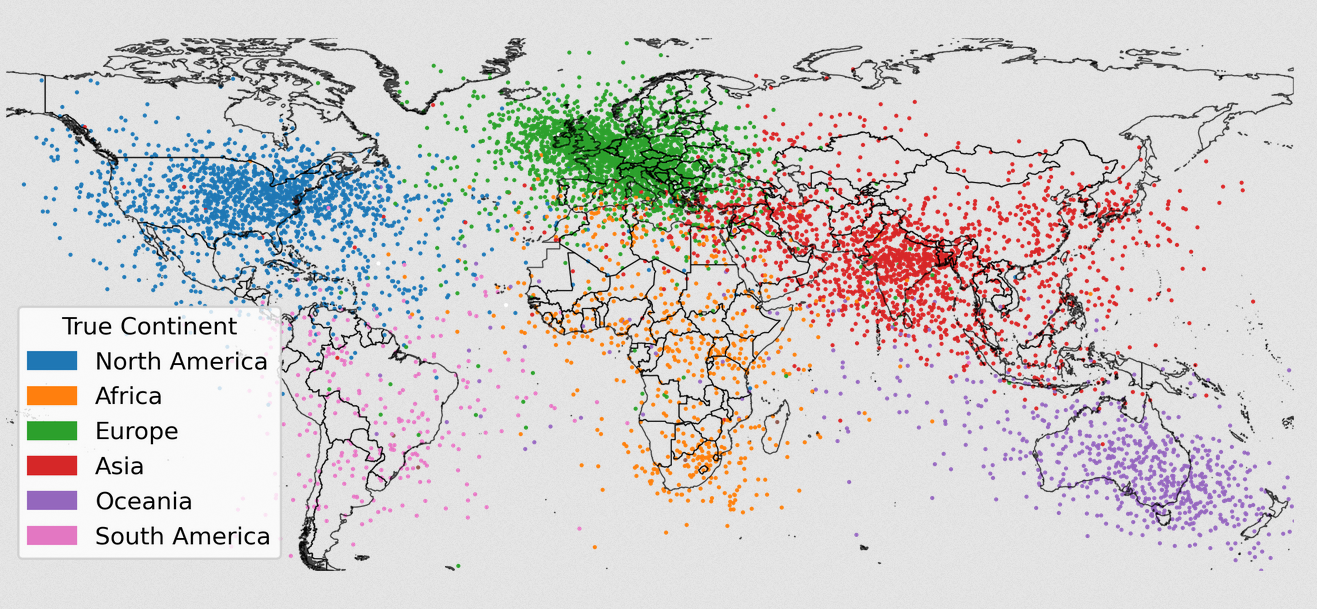
\includegraphics[width=\linewidth, keepaspectratio]{ai_approx_world.png}\\
      {\scriptsize\color{gray}Approximative Weltkarte aus 2 internen Dimensionen eines LLM}
    \end{center}
  \end{columns}

  \quelle{Gurnee, Tegmark. arXiv:2310.02207 (2023)}
\end{frame}

% ── Manifold animation: content defined once, spread across slides ──

% ── Manifold animation: content defined once, spread across slides ──

% Define the text content ONCE here (edit in one place):
\newcommand{\manifoldtitle}{Mannigfaltigkeiten – Übersetzung als Geometrie}
\newcommand{\manifolditems}{%
  \begin{itemize}
    \stich{Sprachen bilden \textbf{Mannigfaltigkeiten} im Embedding-Raum}
    \stich{Japanisch \& Englisch: ähnliche \textbf{Form}, aber verschoben \& gedreht}
    \stich{\textbf{Translation + Rotation} = Übersetzung zwischen Sprachen}
    \stich{Geometrische Transformation statt Wort-für-Wort-Zuordnung}
    \stich{Evidenz: lineare Abbildungen zwischen Sprachräumen
           funktionieren erstaunlich gut\\
           {\small (Mikolov et al.\ 2013)}}
  \end{itemize}
}
\newcommand{\manifoldcaption}{%
  {\scriptsize\color{gray}Animation: Japanische \& englische Wort-Mannigfaltigkeiten,\\
   verbunden durch Translation + Rotation}%
}
\newcommand{\manifoldbox}{%
  \begin{center}
    \colorbox{dunkel!10}{%
      \parbox{0.85\textwidth}{\centering\small
        \textbf{Kernidee:} Die Struktur der Bedeutung ist \emph{sprachunabhängig} –
        nur die \textbf{Einbettung} (Position \& Orientierung der Mannigfaltigkeit) unterscheidet sich.
      }%
    }
  \end{center}
}

% Total number of frames (edit here if you add/remove images):
\newcommand{\manifoldtotalframes}{8}

% Now generate one Beamer frame per image file (8 slides):
\foreach \n in {1,...,8} {%
  \begingroup
  % Zero-pad the number to 3 digits
  \ifnum\n<10
    \def\paddednum{00\the\numexpr\n\relax}%
  \else
    \ifnum\n<100
      \def\paddednum{0\the\numexpr\n\relax}%
    \fi
  \fi
  \begin{frame}[noframenumbering]{\manifoldtitle}
    \begin{columns}[T]
      \column{0.55\textwidth}
      \manifolditems

      \column{0.4\textwidth}
      \begin{center}
        \includegraphics[width=\textwidth]{frames/frames_\paddednum.png}\\[0.3em]
        \manifoldcaption

        % ── Progress bar ──
        \vspace{0.4em}
        \begin{tikzpicture}
          \pgfmathsetmacro{\progress}{\n / \manifoldtotalframes}
          \def\barwidth{3.2}  % cm total width
          \def\barheight{0.18} % cm height

          % Background (gray track)
          \fill[gray!25, rounded corners=1.5pt]
            (0,0) rectangle (\barwidth, \barheight);

          % Filled portion (accent color)
          \fill[akzent, rounded corners=1.5pt]
            (0,0) rectangle (\progress*\barwidth, \barheight);

          % Frame counter text
          \node[font=\tiny\color{gray}, anchor=west] at (\barwidth + 0.15, \barheight/2)
            {\n/\manifoldtotalframes};
        \end{tikzpicture}
      \end{center}
    \end{columns}

    \medskip
    \manifoldbox
  \end{frame}
  \endgroup
}

% ============================================================
\section{Dense Layer – die Grundbausteine}
% ============================================================

\abschnitt{Schritt 1}{Dense Layer – die Grundbausteine}

% ── Was ist ein Dense Layer? ───────────────────────────────
\begin{frame}{Dense Layer – Grundidee}
  \begin{center}
    \colorbox{dunkel!10}{%
      \parbox{0.5\textwidth}{%
        \centering
        $\displaystyle f(\mathbf{x}) = A\,\mathbf{x} + \mathbf{b}$%
      }%
    }
  \end{center}
  \begin{itemize}
    \stich{$A$ = Gewichtsmatrix (Tensor), $\mathbf{b}$ = Bias-Vektor}
    \stich{Jeder Eingang mit jedem Ausgang verbunden}
    \stich{Lineare Transformation: Drehen, Strecken, Verschieben}
  \end{itemize}

  \begin{center}
    
\includegraphics[width=0.35\textwidth]{dense.png}
  \end{center}
\end{frame}

% ── Verschachtelung ────────────────────────────────────────
\begin{frame}{Verschachtelung – warum reicht \emph{eine} Schicht nicht?}
  Zwei Dense Layer hintereinander:
  \formelbox{g(f(\mathbf{x})) = A_2\,(A_1\,\mathbf{x} + \mathbf{b}_1) + \mathbf{b}_2
             = \underbrace{A_2 A_1}_{=\,A'}\,\mathbf{x}
             + \underbrace{A_2\mathbf{b}_1 + \mathbf{b}_2}_{=\,\mathbf{b}'}}
  \begin{center}
    \color{highlight}\textbf{Kollabiert zu einer einzigen linearen Abbildung!}
  \end{center}
  \begin{itemize}
    \stich{Egal wie viele Schichten → bleibt $f(\mathbf{x})=A'\mathbf{x}+\mathbf{b}'$}
    \stich{Tiefe bringt \textbf{nichts} ohne Nichtlinearität}
  \end{itemize}
\end{frame}

% ── Aktivierungsfunktionen ─────────────────────────────────
\begin{frame}{Aktivierungsfunktionen – der Trick}
  \begin{columns}[T]
    \column{0.55\textwidth}
    \formelbox{h(\mathbf{x}) = \sigma\!\bigl(A\,\mathbf{x}+\mathbf{b}\bigr)}
    \begin{itemize}
      \stich{$\sigma$ = nichtlineare Funktion (ReLU, Sigmoid, Tanh, \ldots)}
      \stich{Bricht die Linearität auf}
      \stich{Jetzt: $g(\sigma(f(\mathbf{x}))) \neq A'\mathbf{x}+\mathbf{b}'$}
    \end{itemize}

    \medskip
    \begin{center}
      \textbf{Dense + Nichtlinearität + Dense}\\
      $\Rightarrow$ \emph{universeller Approximator}\\[0.3em]
      {\small (Cybenko 1989, Hornik 1991)}
    \end{center}

    \column{0.4\textwidth}
    % --- Kleine TikZ-Skizze der Aktivierungsfunktionen ---
    \begin{tikzpicture}[scale=0.6, every node/.style={font=\scriptsize}]
      % ReLU
      \draw[->] (-2,0) -- (2.5,0) node[right]{$x$};
      \draw[->] (0,-0.5) -- (0,2.5) node[above]{ReLU};
      \draw[thick, akzent] (-2,0) -- (0,0) -- (2,2);
      % Sigmoid
      \begin{scope}[yshift=-3.5cm]
        \draw[->] (-2,0) -- (2.5,0) node[right]{$x$};
        \draw[->] (0,-0.5) -- (0,2) node[above]{Sigmoid};
        \draw[thick, hell, domain=-2:2.3, samples=50]
          plot (\x, {1.5/(1+exp(-2*\x))});
      \end{scope}
    \end{tikzpicture}
  \end{columns}
\end{frame}

% ── Neue Folie: Universelle Approximation durch ReLU-Knicke ──
% ══════════════════════════════════════════════════════════════
% Approximation – schrittweiser Aufbau (6 Folien)
% ══════════════════════════════════════════════════════════════

% Hilfsmakro für einheitliche Achsen und Clip
\newcommand{\approxaxes}{%
  \clip (-0.7,-1.8) rectangle (7.8,4.5);
  \draw[-{Stealth}] (-0.5,0) -- (7.5,0) node[right]{$x$};
  \draw[-{Stealth}] (0,-1.5) -- (0,4.2) node[above]{$y$};
}
% Zielfunktion (Makro für Konsistenz)
\newcommand{\targetfn}[1][1]{%
  \draw[thick, dunkel, domain=0:7, samples=100, opacity=#1]
    plot (\x, {0.5*sin(70*\x) + 0.06*\x*\x + 0.8});
}

% ══════════════════════════════════════════════════════════════
% BESSER: Komplett saubere Version mit konkreten Werten
% ══════════════════════════════════════════════════════════════

% ── Folie 1: Nur die Zielfunktion ──────────────────────────
\begin{frame}{Wie approximiert ein Netz eine Funktion?}
  \begin{center}
    \begin{tikzpicture}[
        scale=0.85,
        every node/.style={font=\scriptsize},
      ]
      \clip (-0.7,-1.8) rectangle (7.8,4.5);
      \draw[-{Stealth}] (-0.5,0) -- (7.5,0) node[right]{$x$};
      \draw[-{Stealth}] (0,-1.5) -- (0,4.2) node[above]{$y$};

      % Zielfunktion
      \draw[thick, dunkel, domain=0:7, samples=100]
        plot (\x, {0.5*sin(70*\x) + 0.06*\x*\x + 0.8})
        node[right] {$f(x)$};
    \end{tikzpicture}
  \end{center}

  \vfill
  \begin{center}
    \colorbox{dunkel!10}{%
      \parbox{0.75\textwidth}{\centering\small
        Gegeben: eine beliebige stetige Funktion.\\[3pt]
        \textbf{Ziel:} mit einfachen Bausteinen annähern.
      }%
    }
  \end{center}
\end{frame}

% ── Folie 2: Erstes Neuron h₁ ─────────────────────────────
\begin{frame}{Wie approximiert ein Netz eine Funktion?}
  \begin{center}
    \begin{tikzpicture}[
        scale=0.85,
        every node/.style={font=\scriptsize},
      ]
      \clip (-0.7,-1.8) rectangle (7.8,4.5);
      \draw[-{Stealth}] (-0.5,0) -- (7.5,0) node[right]{$x$};
      \draw[-{Stealth}] (0,-1.5) -- (0,4.2) node[above]{$y$};

      % Zielfunktion (blass)
      \draw[thick, dunkel, domain=0:7, samples=100, opacity=0.2]
        plot (\x, {0.5*sin(70*\x) + 0.06*\x*\x + 0.8});

      % h₁: ReLU ab x=0, Steigung +0.9
      % h₁(x) = 0.9 · ReLU(x - 0) = 0.9x für x>0
      \draw[thick, akzent]
        (-0.5, 0) -- (0, 0);
      \draw[thick, akzent]
        (0, 0) -- (7, 3.15);
      \fill[akzent] (0, 0) circle (3pt);
      \node[akzent, above left, font=\small\bfseries] at (1.5, 0.7) {$h_1$};

      % Summe = h₁ + Bias (0.8)
      \draw[line width=2.5pt, akzent!70!black]
        (0, 0.8) -- (7, 3.95);
      \node[akzent!70!black, right, font=\small\bfseries] at (7, 3.95) {$\hat{f}$};
    \end{tikzpicture}
  \end{center}

  \vfill
  \begin{center}
    \colorbox{dunkel!10}{%
      \parbox{0.78\textwidth}{\centering\small
        \textbf{Ein Neuron:} \;
        $h_1(x) = a_1 \cdot \operatorname{ReLU}(x - c_1)$\\[4pt]
        Links vom Knick $c_1$: Ausgabe $= 0$.\\
        Rechts vom Knick: lineare Steigung $a_1$.
      }%
    }
  \end{center}
\end{frame}

% ── Folie 3: Zweites Neuron h₂ ────────────────────────────
\begin{frame}{Wie approximiert ein Netz eine Funktion?}
  \begin{center}
    \begin{tikzpicture}[
        scale=0.85,
        every node/.style={font=\scriptsize},
      ]
      \clip (-0.7,-1.8) rectangle (7.8,4.5);
      \draw[-{Stealth}] (-0.5,0) -- (7.5,0) node[right]{$x$};
      \draw[-{Stealth}] (0,-1.5) -- (0,4.2) node[above]{$y$};

      % Zielfunktion (blass)
      \draw[thick, dunkel, domain=0:7, samples=100, opacity=0.2]
        plot (\x, {0.5*sin(70*\x) + 0.06*\x*\x + 0.8});

      % h₁ (blass)
      \draw[thick, akzent, dashed, opacity=0.3]
        (0, 0) -- (7, 3.15);
      \node[akzent, opacity=0.4, above left] at (1.5, 0.7) {$h_1$};

      % h₂: ReLU ab x=1.5, Steigung -1.5
      % h₂(x) = -1.5 · ReLU(x - 1.5)
      \draw[thick, hell]
        (-0.5, 0) -- (1.5, 0);
      \draw[thick, hell]
        (1.5, 0) -- (7, -8.25);  % wird geclippt
      \fill[hell] (1.5, 0) circle (3pt);
      \node[hell, below right, font=\small\bfseries] at (2.0, -0.5) {$h_2$};

      % Summe: bias + h₁ + h₂
      % x<0: 0.8, 0<x<1.5: 0.8 + 0.9x, x>1.5: 0.8 + 0.9x - 1.5(x-1.5)
      % x>1.5: 0.8 + 0.9x - 1.5x + 2.25 = 3.05 - 0.6x
      \draw[line width=2.5pt, akzent!70!black]
        (0, 0.8) -- (1.5, 2.15) -- (7, -1.15);
      % Clip rettet uns – nur sichtbarer Teil
      \foreach \kx/\ky in {1.5/2.15} {
        \fill[akzent!70!black] (\kx, \ky) circle (3pt);
      }
      \node[akzent!70!black, above right, font=\small\bfseries] at (0.3, 1.5) {$\hat{f}$};
    \end{tikzpicture}
  \end{center}

  \vfill
  \begin{center}
    \colorbox{dunkel!10}{%
      \parbox{0.78\textwidth}{\centering\small
        \textbf{Zweites Neuron} $h_2$ mit \textbf{negativem} Gewicht.\\[4pt]
        Die Summe knickt jetzt ab – die Steigung ändert sich.
      }%
    }
  \end{center}
\end{frame}

% ── Folie 4: Drittes Neuron h₃ ────────────────────────────
\begin{frame}{Wie approximiert ein Netz eine Funktion?}
  \begin{center}
    \begin{tikzpicture}[
        scale=0.85,
        every node/.style={font=\scriptsize},
      ]
      \clip (-0.7,-1.8) rectangle (7.8,4.5);
      \draw[-{Stealth}] (-0.5,0) -- (7.5,0) node[right]{$x$};
      \draw[-{Stealth}] (0,-1.5) -- (0,4.2) node[above]{$y$};

      % Zielfunktion (blass)
      \draw[thick, dunkel, domain=0:7, samples=100, opacity=0.2]
        plot (\x, {0.5*sin(70*\x) + 0.06*\x*\x + 0.8});

      % h₁, h₂ (blass)
      \draw[thick, akzent, dashed, opacity=0.2]
        (0, 0) -- (7, 3.15);
      \draw[thick, hell, dashed, opacity=0.2]
        (1.5, 0) -- (7, -8.25);

      % h₃: ReLU ab x=3.0, Steigung +1.2
      \draw[thick, highlight]
        (-0.5, 0) -- (3.0, 0);
      \draw[thick, highlight]
        (3.0, 0) -- (7, 4.8);
      \fill[highlight] (3.0, 0) circle (3pt);
      \node[highlight, above left, font=\small\bfseries] at (4.5, 1.5) {$h_3$};

      % Summe: bias + h₁ + h₂ + h₃
      % x in [0,1.5]: 0.8 + 0.9x
      % x in [1.5,3.0]: 3.05 - 0.6x
      % x in [3.0,7]: 3.05 - 0.6x + 1.2(x-3.0) = -0.55 + 0.6x
      \draw[line width=2.5pt, akzent!70!black]
        (0, 0.8) -- (1.5, 2.15) -- (3.0, 1.25) -- (7, 3.65);
      \foreach \kx/\ky in {1.5/2.15, 3.0/1.25} {
        \fill[akzent!70!black] (\kx, \ky) circle (3pt);
      }
      \node[akzent!70!black, right, font=\small\bfseries] at (7, 3.65) {$\hat{f}$};
    \end{tikzpicture}
  \end{center}

  \vfill
  \begin{center}
    \colorbox{dunkel!10}{%
      \parbox{0.78\textwidth}{\centering\small
        \textbf{Drittes Neuron} $h_3$ – Steigung wird wieder positiv.\\[4pt]
        Zwei Knicke – die Summe folgt der Kurve besser.
      }%
    }
  \end{center}
\end{frame}

% ── Folie 5: Viertes Neuron h₄ (korrigiert – geht nach oben) ──
\begin{frame}{Wie approximiert ein Netz eine Funktion?}
  \begin{center}
    \begin{tikzpicture}[
        scale=0.85,
        every node/.style={font=\scriptsize},
      ]
      \clip (-0.7,-1.8) rectangle (7.8,4.5);
      \draw[-{Stealth}] (-0.5,0) -- (7.5,0) node[right]{$x$};
      \draw[-{Stealth}] (0,-1.5) -- (0,4.2) node[above]{$y$};

      % Zielfunktion (etwas kräftiger)
      \draw[thick, dunkel, domain=0:7, samples=100, opacity=0.35]
        plot (\x, {0.5*sin(70*\x) + 0.06*\x*\x + 0.8});
      \node[dunkel, right, opacity=0.7] at (7, 3.5) {$f(x)$};

      % h₁, h₂, h₃ (blass)
      \draw[thick, akzent, dashed, opacity=0.15]  (0, 0) -- (7, 3.15);
      \draw[thick, hell, dashed, opacity=0.15]    (1.5, 0) -- (7, -8.25);
      \draw[thick, highlight, dashed, opacity=0.15] (3.0, 0) -- (7, 4.8);

      % h₄: ReLU ab x=5.0, Steigung +0.6 (positiv! → geht nach oben)
      \draw[thick, violet]
        (-0.5, 0) -- (5.0, 0);
      \draw[thick, violet]
        (5.0, 0) -- (7, 1.2);
      \fill[violet] (5.0, 0) circle (3pt);
      \node[violet, above right, font=\small\bfseries] at (5.5, 0.5) {$h_4$};

      % Summe: bias + h₁ + h₂ + h₃ + h₄
      % x in [0,1.5]: 0.8 + 0.9x
      % x in [1.5,3.0]: 3.05 - 0.6x
      % x in [3.0,5.0]: -0.55 + 0.6x
      % x in [5.0,7]: -0.55 + 0.6x + 0.6(x-5.0) = -3.55 + 1.2x
      %   bei x=5.0: -3.55 + 6.0 = 2.45
      %   bei x=7.0: -3.55 + 8.4 = 4.85 → wird geclippt, aber passt zur steigenden fkt
      \draw[line width=2.5pt, akzent!70!black]
        (0, 0.8) -- (1.5, 2.15) -- (3.0, 1.25) -- (5.0, 2.45) -- (7, 4.85);
      \foreach \kx/\ky in {1.5/2.15, 3.0/1.25, 5.0/2.45} {
        \fill[akzent!70!black] (\kx, \ky) circle (3pt);
      }
      \node[akzent!70!black, right, font=\small\bfseries] at (7, 4.2) {$\hat{f}$};
    \end{tikzpicture}
  \end{center}

  \vfill
  \begin{center}
    \colorbox{dunkel!10}{%
      \parbox{0.78\textwidth}{\centering\small
        \textbf{Viertes Neuron} $h_4$ – verstärkt die Steigung am Ende.\\[4pt]
        Drei Knicke, vier Segmente – die Form stimmt schon grob.
      }%
    }
  \end{center}
\end{frame}

% ── Folie 6: Fazit – viele Neuronen (korrigiert) ───────────────────────
\begin{frame}{Wie approximiert ein Netz eine Funktion?}
  \begin{center}
    \begin{tikzpicture}[
        scale=0.85,
        every node/.style={font=\scriptsize},
      ]
      \clip (-0.7,-1.8) rectangle (7.8,4.5);
      \draw[-{Stealth}] (-0.5,0) -- (7.5,0) node[right]{$x$};
      \draw[-{Stealth}] (0,-1.5) -- (0,4.2) node[above]{$y$};

      % Zielfunktion
      \draw[thick, dunkel, domain=0:7, samples=100]
        plot (\x, {0.5*sin(70*\x) + 0.06*\x*\x + 0.8})
        node[right] {$f(x)$};

      % Grobe Approximation (4 Neuronen – jetzt passend zu Folie 5)
      \draw[line width=1.5pt, akzent!70!black, opacity=0.35]
        (0, 0.8) -- (1.5, 2.15) -- (3.0, 1.25) -- (5.0, 2.45) -- (7, 4.85);
      \node[akzent!70!black, opacity=0.5, font=\tiny, above] at (1.0, 2.3) {4 Neuronen};

      % Feine Approximation (simuliert mit vielen Samples)
      \draw[line width=2pt, highlight, domain=0:7, samples=25]
        plot (\x, {0.5*sin(70*\x) + 0.06*\x*\x + 0.8});
      \node[highlight, font=\tiny, above] at (5.5, 3.8) {viele Neuronen};
    \end{tikzpicture}
  \end{center}

  \vfill
  \begin{center}
    \colorbox{dunkel!10}{%
      \parbox{0.82\textwidth}{\centering
        \textbf{Jedes Neuron} = ein Knick = eine Richtungsänderung.\\[5pt]
        Mehr Neuronen $\;\longrightarrow\;$ mehr Knicke $\;\longrightarrow\;$ beliebig genaue Annäherung.\\[5pt]
        {\small Das ist der Kern des \textbf{universellen Approximationssatzes}.}
      }%
    }
  \end{center}
\end{frame}

% ── Black Box ──────────────────────────────────────────────
\begin{frame}{Black Box – wir sehen nur Input \& Output}
  \begin{center}
    \begin{tikzpicture}[
        box/.style={draw, thick, rounded corners, minimum width=3cm,
                     minimum height=1.5cm, fill=dunkel, text=white,
                     font=\large\bfseries},
        arr/.style={-{Stealth[length=5mm]}, thick, akzent}
      ]
      \node (in)  at (-4,0) {\Large Eingabe};
      \node[box] (nn) at (0,0) {?};
      \node (out) at (4,0) {\Large Ausgabe};
      \draw[arr] (in) -- (nn);
      \draw[arr] (nn) -- (out);
    \end{tikzpicture}
  \end{center}
  \begin{itemize}
    \stich{Netzwerk lernt \emph{interne Muster} – wir sehen sie nicht direkt}
    \stich{Kann jedes stetige Problem approximieren …}
    \stich{… versteht aber nicht \emph{warum}}
  \end{itemize}
\end{frame}

% ── Beispiel: Gartenbewässerung ───────────────────────────
\begin{frame}{Beispiel: Gartenbewässerungs-KI}
  \textbf{Ziel:} Ernte maximieren \quad
  \textbf{Eingabe:} Bewässerungszeitpunkte

  \medskip
  \begin{center}
  \small
  \begin{tabular}{lcccc}
    \toprule
    \textbf{Zeitfenster} & \textbf{Erdbeeren} & \textbf{Kartoffeln}
      & \textbf{Tomaten} & \textbf{Zucchini} \\
    & (kg) & (kg) & (kg) & (kg) \\
    \midrule
    06:00 – 08:00  & 12{,}4 & 38{,}1 & 9{,}7  & 15{,}2 \\
    12:00 – 14:00  &  7{,}1 & 33{,}5 & 5{,}2  & 12{,}8 \\
    18:00 – 20:00  & 11{,}9 & 37{,}4 & 9{,}3  & 14{,}9 \\
    23:00 – 02:00  &  4{,}3 & 28{,}6 & 4{,}1  &  9{,}7 \\
    \rowcolor{highlight!15}
    \textbf{Optimal (KI)} & \textbf{13{,}1} & \textbf{39{,}2}
      & \textbf{10{,}4} & \textbf{16{,}0} \\
    \bottomrule
  \end{tabular}
  \end{center}
\end{frame}

% ── Warum nachts schlecht? ─────────────────────────────────
\begin{frame}{Versteckte Zusammenhänge}
  \begin{columns}[T]
    \column{0.55\textwidth}
    \begin{itemize}
      \stich{\textbf{Nachts wässern?}\\
             Schnecken aktiver bei Nässe → fressen Ernte ab}
      \stich{\textbf{Wind egal?}\\
             Mehr Wind → mehr Verdunstung}
      \stich{\textbf{Mittags wässern?}\\
             Wassertropfen = Linsen → Sonnenbrand auf Blättern}
    \end{itemize}

    \medskip
    \color{akzent}\textbf{→ KI lernt: ``nachts/mittag/... = schlechter Ertrag''}\\
    \color{gray}\textit{Weiß aber nicht, dass Schnecken/Wind/Wassertropfenlinsen der Grund sind.}

    \column{0.4\textwidth}
        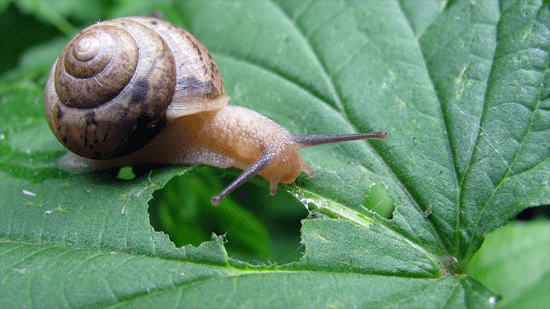
\includegraphics[width=\textwidth]{snails.png}

        \vspace{0.5em}
        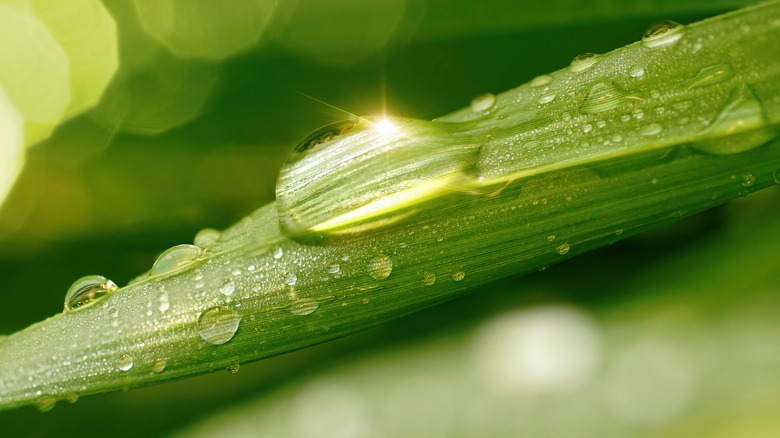
\includegraphics[width=\textwidth]{water_droplet.jpg}
  \end{columns}
\end{frame}

% ── Verschachtelung als Diagramm ──────────────────────────
\begin{frame}{Verschachtelte Layer = Abstraktion}
  \begin{center}
    \begin{tikzpicture}[
        layer/.style={draw, thick, rounded corners, minimum width=2.2cm, 
                     minimum height=0.8cm, font=\small\bfseries},
        arr/.style={-{Stealth}, thick},
        note/.style={font=\scriptsize, text=gray, anchor=north},
        node distance=0.6cm
      ]
      % Nodes von links nach rechts
      \node (in) {\footnotesize $\mathbf{x}$};
      
      \node[layer, fill=hell!20, right=of in]    (l1) {$f$};
      \node[right=0.3cm of l1] (z1) {\footnotesize $z_1$};
      
      \node[layer, fill=akzent!20, right=0.3cm of z1]  (s1) {$\sigma$};
      \node[right=0.3cm of s1] (z2) {\footnotesize $z_2$};
      
      \node[layer, fill=hell!20, right=0.3cm of z2]    (l2) {$g$};
      \node[right=of l2] (out) {\footnotesize $\hat{y}$};

      % Pfeile
      \draw[arr] (in) -- (l1);
      \draw[arr] (l1) -- (z1);
      \draw[arr] (z1) -- (s1);
      \draw[arr] (s1) -- (z2);
      \draw[arr] (z2) -- (l2);
      \draw[arr] (l2) -- (out);

      % Beschriftungen unten
      \node[note] at (l1.south) [below=0.1cm] {Dense Layer 1};
      \node[note] at (s1.south) [below=0.1cm] {ReLU};
      \node[note] at (l2.south) [below=0.1cm] {Dense Layer 2};
    \end{tikzpicture}
  \end{center}

  \vspace{0.3cm}
  \begin{columns}[T]
    \begin{column}{0.45\textwidth}
      \textbf{Eingabe:}\\[0.1cm]
      \small
      $x_1$ = Temperatur\\
      $x_2$ = Uhrzeit\\
      $x_3$ = Windgeschwindigkeit\\
      $\vdots$
    \end{column}
    \begin{column}{0.55\textwidth}
      \textbf{Vorwärtsdurchlauf:}\\[0.1cm]
      \small
      $z_1 = f(\mathbf{x}) = A\mathbf{x} + \mathbf{b}$\\
      $z_2 = \sigma(z_1)$\\
      $\hat{y} = g(z_2) = C\,z_2 + \mathbf{d}$
    \end{column}
  \end{columns}

  \vspace{0.3cm}
  \begin{itemize}
    \stich{Ohne $\sigma$: alles kollabiert zu \emph{einer} linearen Abbildung}
    \stich{Mit $\sigma$: jede Schicht lernt \textbf{abstraktere Merkmale}}
  \end{itemize}
\end{frame}

\section{Positional Encoding}
% ============================================================

\abschnitt{Schritt 2}{Positional Encoding}

\begin{frame}{Positional Encoding – Wo steht ein Wort?}
  \formelbox{\text{PE}_{(\text{pos},\,2i)} = \sin\!\Bigl(\frac{\text{pos}}{10000^{2i/d}}\Bigr),
             \qquad
             \text{PE}_{(\text{pos},\,2i+1)} = \cos\!\Bigl(\frac{\text{pos}}{10000^{2i/d}}\Bigr)}

  \begin{itemize}
    \stich{Jede Position bekommt ein \textbf{einzigartiges Muster} aus Sinus-/Cosinus-Wellen}
    \stich{Wird auf den Wortvektor \textbf{addiert} (nicht konkateniert)}
    \stich{Hochdimensionale ``Spirale'' um jedes Wort}
    \stich{Wort $\neq$ einzelner Punkt, sondern eine \textbf{Gegend} im Raum}
    \stich{Relative Positionen → Beziehungen zwischen Wörtern}
  \end{itemize}
\end{frame}

\begin{frame}[plain]
  \definecolor{dim1}{HTML}{E8590C}
  \definecolor{dim2}{HTML}{0F3460}
  \definecolor{dim3}{HTML}{E94560}
  \definecolor{dim4}{HTML}{1A8F3C}
  \definecolor{dim5}{HTML}{7B2D8B}
  \definecolor{dim6}{HTML}{D4A017}

  \centering
  \foreach \pos in {0,1,...,19} {%
    \only<\the\numexpr\pos+1\relax>{%
      \begin{tikzpicture}
        \useasboundingbox (-5.2,-5.5) rectangle (5.2,5.2);
        \fill[white] (-5.2,-5.5) rectangle (5.2,5.2);

        % Winkel
        \pgfmathsetmacro{\aA}{36*\pos}
        \pgfmathsetmacro{\aB}{24*\pos}
        \pgfmathsetmacro{\aC}{16*\pos}
        \pgfmathsetmacro{\aD}{10*\pos}
        \pgfmathsetmacro{\aE}{6*\pos}
        \pgfmathsetmacro{\aF}{3*\pos}

        % Referenzlinien
        \draw[gray!12, thin] (0,0) -- (0:4.7);
        \draw[gray!12, thin] (0,0) -- (90:4.7);
        \draw[gray!12, thin] (0,0) -- (180:4.7);
        \draw[gray!12, thin] (0,0) -- (270:4.7);

        % Kreise
        \draw[dim1, thick, opacity=0.5] (0,0) circle (1.0);
        \draw[dim2, thick, opacity=0.45] (0,0) circle (1.7);
        \draw[dim3, thick, opacity=0.4] (0,0) circle (2.4);
        \draw[dim4, thick, opacity=0.35] (0,0) circle (3.1);
        \draw[dim5, thick, opacity=0.3] (0,0) circle (3.8);
        \draw[dim6, thick, opacity=0.25] (0,0) circle (4.5);

        % Labels
        \node[font=\tiny, dim1] at (200:1.25) {\tiny$(d_0,d_1)$};
        \node[font=\tiny, dim2] at (200:1.95) {\tiny$(d_2,d_3)$};
        \node[font=\tiny, dim3] at (200:2.65) {\tiny$(d_4,d_5)$};
        \node[font=\tiny, dim4] at (200:3.35) {\tiny$(d_6,d_7)$};
        \node[font=\tiny, dim5] at (200:4.05) {\tiny$(d_8,d_9)$};
        \node[font=\tiny, dim6] at (200:4.8) {\tiny$(d_{10},d_{11})$};

        % Verbindungslinien
        \draw[gray, thin, opacity=0.15] (0,0) -- (\aA:1.0);
        \draw[gray, thin, opacity=0.12] (0,0) -- (\aB:1.7);
        \draw[gray, thin, opacity=0.1] (0,0) -- (\aC:2.4);
        \draw[gray, thin, opacity=0.08] (0,0) -- (\aD:3.1);
        \draw[gray, thin, opacity=0.06] (0,0) -- (\aE:3.8);
        \draw[gray, thin, opacity=0.04] (0,0) -- (\aF:4.5);

        % Spur
        \ifnum\pos>0\relax
          \draw[dim1, thick, opacity=0.15] (0:1.0) arc (0:\aA:1.0);
          \draw[dim2, thick, opacity=0.15] (0:1.7) arc (0:\aB:1.7);
          \draw[dim3, thick, opacity=0.15] (0:2.4) arc (0:\aC:2.4);
          \draw[dim4, thick, opacity=0.15] (0:3.1) arc (0:\aD:3.1);
          \draw[dim5, thick, opacity=0.15] (0:3.8) arc (0:\aE:3.8);
          \draw[dim6, thick, opacity=0.15] (0:4.5) arc (0:\aF:4.5);
        \fi

        % Glow
        \fill[dim1, opacity=0.12] (\aA:1.0) circle (8pt);
        \fill[dim2, opacity=0.12] (\aB:1.7) circle (8pt);
        \fill[dim3, opacity=0.12] (\aC:2.4) circle (8pt);
        \fill[dim4, opacity=0.12] (\aD:3.1) circle (8pt);
        \fill[dim5, opacity=0.12] (\aE:3.8) circle (8pt);
        \fill[dim6, opacity=0.12] (\aF:4.5) circle (8pt);

        % Punkte
        \fill[dim1] (\aA:1.0) circle (4pt);
        \fill[dim2] (\aB:1.7) circle (4pt);
        \fill[dim3] (\aC:2.4) circle (4pt);
        \fill[dim4] (\aD:3.1) circle (4pt);
        \fill[dim5] (\aE:3.8) circle (4pt);
        \fill[dim6] (\aF:4.5) circle (4pt);

        % Startpunkte
        \foreach \r in {1.0, 1.7, 2.4, 3.1, 3.8, 4.5} {
          \draw[gray!40] (0:\r) circle (1.5pt);
        }

        % Wort
        \fill[white] (0,0) circle (0.6);
        \node[draw, thick, rounded corners=3pt, fill=black!85, text=white,
              minimum width=1.2cm, minimum height=0.5cm,
              font=\small\bfseries] at (0,0) {Katze};

        % Position
        \node[font=\large\bfseries, anchor=north west] at (-5.0, 5.0)
          {pos = \pos};

        % Legende
        \node[anchor=north east, font=\tiny, text width=2.5cm, align=left,
              fill=white, draw=gray!30, rounded corners, inner sep=2pt]
          at (5.0, 5.0) {%
          \textcolor{dim1}{$\bullet$ schnell}\\
          \textcolor{dim2}{$\bullet$}\\
          \textcolor{dim3}{$\bullet$}\\
          \textcolor{dim4}{$\bullet$}\\
          \textcolor{dim5}{$\bullet$}\\
          \textcolor{dim6}{$\bullet$ langsam}
        };

      \end{tikzpicture}%
    }%
  }%
\end{frame}

% ============================================================
\section{Der große Überblick – Token-Vorhersage}
% ============================================================

\abschnitt{Schritt 3a}{Das Gesamtbild – Token-Vorhersage}

\begin{frame}{Wie ein Sprachmodell Text generiert}
  \begin{center}
    \begin{tikzpicture}[
        box/.style={draw, thick, rounded corners, minimum width=2.2cm,
                     minimum height=0.9cm, font=\scriptsize\bfseries,
                     text width=2.0cm, align=center},
        arr/.style={-{Stealth}, thick, akzent},
        node distance=0.4cm
      ]
      \node[box, fill=hell!15]      (tok) {Tokenisierung};
      \node[box, fill=hell!15, right=of tok] (pe)  {+ Pos.\ Encoding};
      \node[box, fill=dunkel!15, right=of pe]  (layers) {Layer $\times N$};
      \node[box, fill=highlight!15, right=of layers] (winkel) {Winkel-\\vergleich};
      \node[box, fill=akzent!15, right=of winkel] (topk) {Top-$k$\\+ Temp.};

      \draw[arr] (tok) -- (pe);
      \draw[arr] (pe) -- (layers);
      \draw[arr] (layers) -- (winkel);
      \draw[arr] (winkel) -- (topk);

      % Rückpfeil
      \draw[arr, dashed, gray] (topk.south) -- ++(0,-0.8)
        -| node[below, pos=0.25, font=\scriptsize\color{gray}]
           {gewähltes Token → zurück an Eingabe} (tok.south);
    \end{tikzpicture}
  \end{center}

  \begin{itemize}
    \stich{Layer passen \textbf{Winkel} zwischen Token-Vektoren an}
    \stich{Am Ende: Winkel zu \emph{allen} bekannten Tokens vergleichen}
    \stich{Top-$k$ Kandidaten → \textbf{zufällig} einen wählen}
    \stich{Gewähltes Token wird angehängt → Prozess wiederholen}
  \end{itemize}
\end{frame}

% ── Temperatur ─────────────────────────────────────────────
\begin{frame}{Temperatur – Kreativität vs.\ Sachlichkeit}
  \begin{columns}[T]
    \column{0.55\textwidth}
    \begin{itemize}
      \stich{$T \to 0$: immer das wahrscheinlichste Token → \textbf{sachlich, deterministisch}}
      \stich{$T \to \infty$: gleichverteilte Wahl → \textbf{kreativ, chaotisch}}
      \stich{Name: \textbf{Boltzmann-Verteilung}\\
             {\small Ursprünglich: Geschwindigkeitsverteilung von Gasmolekülen}}
    \end{itemize}

    \column{0.4\textwidth}
    \placeholder[0.9\linewidth]{Bild: Boltzmann + Gasmoleküle}
  \end{columns}
\end{frame}

% ── EOS Token ──────────────────────────────────────────────
\begin{frame}{Wann hört die KI auf?}
  \begin{center}
    \texttt{\color{dunkel}%
      Frage: Was ist 2+2?\\[0.3em]
      Antwort: 4\,\color{highlight}\textbf{<eos>}}
  \end{center}

  \begin{itemize}
    \stich{\texttt{<eos>} = \emph{End of Sequence} – spezielles Token}
    \stich{Genauso gelernt wie alle anderen Tokens}
    \stich{In Trainingsdaten stand es am Ende jeder Antwort}
    \stich{Wenn das Modell \texttt{<eos>} als nächstes Token wählt → \textbf{Generierung stoppt}}
  \end{itemize}
\end{frame}

% ============================================================
\section{Was passiert in den Layern?}
% ============================================================

\abschnitt{Schritt 3b}{Was passiert \emph{in} den Layern?}

% ── Grobe Struktur ─────────────────────────────────────────
\begin{frame}{Zwei Operationen pro Layer}
  \begin{center}
    \begin{tikzpicture}[
        box/.style={draw, thick, rounded corners, minimum width=4cm,
                     minimum height=1.2cm, font=\bfseries},
        arr/.style={-{Stealth}, thick}
      ]
      \node[box, fill=hell!20]      (attn) at (0,2) {Attention};
      \node[box, fill=akzent!20]    (ffn)  at (0,0) {Feed-Forward (Dense + ReLU)};
      \node[font=\small, text width=5.5cm, right=1.5cm of attn]
        {``In welcher \textbf{Beziehung} steht jedes Wort zu allen anderen?''};
      \node[font=\small, text width=5.5cm, right=1.5cm of ffn]
        {``Was mache ich jetzt mit dieser Info + den Positionen?''};
      \draw[arr] (attn) -- (ffn);
    \end{tikzpicture}
  \end{center}

  \medskip
  \begin{itemize}
    \stich{\textbf{Frühe Layer:} konkret – Wortteile zusammenfügen
           (z.\,B.\ \texttt{brave} + \texttt{ly} → Adverb)}
    \stich{\textbf{Späte Layer:} abstrakt – semantische Zusammenhänge,
           kaum noch menschlich interpretierbar}
  \end{itemize}
\end{frame}

% ── Residual Stream ────────────────────────────────────────
\begin{frame}{Der Residual Stream – globales Notizbuch}
  \begin{center}
    \begin{tikzpicture}[
        expert/.style={draw, thick, rounded corners, minimum width=1.5cm,
                        minimum height=0.7cm, fill=hell!20, font=\scriptsize\bfseries},
        arr/.style={-{Stealth}, thick, akzent},
        stream/.style={line width=3pt, dunkel!50}
      ]
      % Residual Stream
      \draw[stream] (0,0) -- (12,0);
      \node[below, font=\small\color{dunkel}] at (6,-0.4) {Residual Stream};

      % Experten-Gruppen (feste Positionen, keine Dezimalen in Namen)
      \node[expert] (eA) at (1.5, 1.2) {L1};
      \node[expert] (eB) at (4, 1.2)   {L2};
      \node[expert] (eC) at (6.5, 1.2) {L3};
      \node[expert] (eD) at (9, 1.2)   {$\ldots$};
      \node[expert] (eE) at (10.5, 1.2){L$_N$};

      % Pfeile hoch und runter
      \foreach \n/\x in {eA/1.5, eB/4, eC/6.5, eD/9, eE/10.5} {
        \draw[arr] (\x, 0.15) -- (\n.south);
        \draw[arr] ([xshift=3mm]\n.south) -- ++(0,-0.95);
      }

      \node[left, font=\small] at (0,0) {Input};
      \node[right, font=\small] at (12,0) {Output};
    \end{tikzpicture}
  \end{center}

  \begin{itemize}
    \stich{Ursprünglich erfunden: tiefe Netze besser trainierbar machen (ResNets)}
    \stich{Hier: \textbf{globales Workbook} -- jede Schicht liest und schreibt darauf}
    \stich{Wie ein Text, der einer Reihe von Experten gegeben wird --
           jeder kritzelt seine Notizen drauf}
    \stich{Hunderte Schichten, hunderte Experten-Runden}
  \end{itemize}
\end{frame}

% ── Attention Heads ────────────────────────────────────────
\begin{frame}{Attention Heads – die Linsen}
  \begin{columns}[T]
    \column{0.55\textwidth}
    \begin{itemize}
      \stich{Jeder Attention Head = eine \textbf{Linse},
             die auf einen bestimmten Aspekt fokussiert}
      \stich{Baut \textbf{Beziehungsstruktur} zwischen Wörtern auf}
      \stich{Ergebnis → an Feed-Forward-Netz (Dense + ReLU)}
      \stich{FFN entscheidet: \emph{wie muss der Raum der nächsten Schicht
             angepasst werden?}}
    \end{itemize}

    \column{0.4\textwidth}
    % Simplizialkomplex-Skizze (Bedeutung "einkringeln")
    \begin{tikzpicture}[scale=0.9]
      % Punkte (Tokens)
      \coordinate (A) at (0,0);
      \coordinate (B) at (2.5,0.3);
      \coordinate (C) at (1.2,2);
      \coordinate (D) at (3.2,1.8);
      \coordinate (E) at (0.5,3.2);

      % 2-Simplex (Dreieck) = "eingekringelte Bedeutung"
      \fill[akzent!15] (A) -- (B) -- (C) -- cycle;
      \fill[hell!15] (B) -- (C) -- (D) -- cycle;

      % Kanten
      \draw[thick, dunkel] (A) -- (B) -- (C) -- cycle;
      \draw[thick, dunkel] (B) -- (D) -- (C);
      \draw[thick, dunkel, dashed] (C) -- (E);
      \draw[thick, dunkel, dashed] (A) -- (E);

      % Knoten
      \foreach \p/\lab in {A/\text{Die}, B/\text{Katze}, C/\text{sitzt},
                            D/\text{auf}, E/\text{dem}} {
        \fill[dunkel] (\p) circle (3pt);
        \node[font=\scriptsize, above=2pt] at (\p) {$\lab$};
      }

      % Annotation
      \node[font=\tiny\color{akzent}, rotate=20] at (1.2, 0.6)
        {Bedeutungsregion};
    \end{tikzpicture}
  \end{columns}

  \medskip
  {\small\color{gray}Simplizialkomplex: Beziehungen zwischen Tokens als
   geometrische Struktur – Bedeutung wird ``eingekringelt''.}
\end{frame}

% ── Attention Head: 3D-Simplizialkomplex (Tetraeder) ───────
\begin{frame}{Attention Head – Bedeutung auf dem 3-Simplex}
  \begin{center}
    \begin{tikzpicture}[
        scale=1.3,
        % Isometrische 3D-Projektion (von Hand)
        x={(-0.45cm,-0.35cm)},   % x-Achse nach links-unten
        y={(0.95cm,0cm)},         % y-Achse nach rechts
        z={(0cm,0.95cm)},         % z-Achse nach oben
      ]

      % ════════════════════════════════════════════════════
      %  TETRAEDER-ECKEN (3-Simplex = 4 Ecken)
      % ════════════════════════════════════════════════════
      \coordinate (V1) at (0, 0, 0);      % vorne-links-unten
      \coordinate (V2) at (0, 4, 0);      % vorne-rechts-unten
      \coordinate (V3) at (4, 2, 0);      % hinten-unten
      \coordinate (V4) at (1, 2, 4);      % oben (Spitze)

      % ════════════════════════════════════════════════════
      %  HINTERE KANTEN (gestrichelt, verdeckt)
      % ════════════════════════════════════════════════════
      \draw[dunkel, thick, dashed, opacity=0.3] (V3) -- (V1);
      \draw[dunkel, thick, dashed, opacity=0.3] (V3) -- (V2);

      % ════════════════════════════════════════════════════
      %  FLÄCHEN (halbtransparent)
      % ════════════════════════════════════════════════════
      % Boden (V1-V2-V3)
      \fill[hell!8, opacity=0.25] (V1) -- (V2) -- (V3) -- cycle;

      % Vordere Fläche links (V1-V2-V4)
      \fill[akzent!10, opacity=0.35] (V1) -- (V2) -- (V4) -- cycle;

      % Rechte Fläche (V2-V3-V4)
      \fill[highlight!8, opacity=0.25] (V2) -- (V3) -- (V4) -- cycle;

      % Linke Fläche (V1-V3-V4)
      \fill[hell!12, opacity=0.2] (V1) -- (V3) -- (V4) -- cycle;

      % ════════════════════════════════════════════════════
      %  VORDERE KANTEN (sichtbar)
      % ════════════════════════════════════════════════════
      \draw[dunkel, line width=1.8pt] (V1) -- (V2);
      \draw[dunkel, line width=1.8pt] (V1) -- (V4);
      \draw[dunkel, line width=1.8pt] (V2) -- (V4);
      \draw[dunkel, line width=1.8pt] (V2) -- (V3);
      \draw[dunkel, line width=1.8pt] (V3) -- (V4);

      % Eckbeschriftung
      \node[font=\tiny\color{dunkel}, below left]  at (V1) {$v_1$};
      \node[font=\tiny\color{dunkel}, below right] at (V2) {$v_2$};
      \node[font=\tiny\color{dunkel}, left]         at (V3) {$v_3$};
      \node[font=\tiny\color{dunkel}, above]        at (V4) {$v_4$};

      % ════════════════════════════════════════════════════
      %  ZENTRUM DES TETRAEDERS
      % ════════════════════════════════════════════════════
      \coordinate (Z) at (1.25, 2, 1);  % Schwerpunkt ≈ Mittel der 4 Ecken
      \fill[dunkel] (Z) circle (1.5pt);

      % ════════════════════════════════════════════════════
      %  TOKEN-PUNKTE IM INNEREN (vor Projektion)
      % ════════════════════════════════════════════════════
      \coordinate (T1) at (0.5, 1.2, 1.0);   % Die
      \coordinate (T2) at (0.8, 2.5, 0.5);   % Katze
      \coordinate (T3) at (1.0, 2.8, 0.8);   % jagt
      \coordinate (T4) at (1.5, 3.0, 1.5);   % die
      \coordinate (T5) at (0.8, 2.2, 2.5);   % Maus

      % Blasse innere Punkte
      \foreach \t/\lab in {T1/Die, T2/Katze, T3/jagt, T4/die, T5/Maus} {
        \fill[gray!35] (\t) circle (1.8pt);
        \node[font=\tiny\color{gray!60}, above=0pt] at (\t) {\lab};
      }

      % ════════════════════════════════════════════════════
      %  PROJIZIERTE PUNKTE AUF DER OBERFLÄCHE
      %  (manuell auf Tetraeder-Flächen gelegt)
      % ════════════════════════════════════════════════════

      % P1: "Die" → linke Fläche (V1-V4-V3)
      \coordinate (P1) at (1.2, 0.6, 2.0);

      % P2: "Katze" → vordere Fläche unten (V1-V2, nahe Boden)
      \coordinate (P2) at (0.1, 1.8, 0.0);

      % P3: "jagt" → vordere Fläche (V1-V2-V4), mittig
      \coordinate (P3) at (0.2, 2.3, 1.2);

      % P4: "die" → rechte Fläche (V2-V3-V4)
      \coordinate (P4) at (1.5, 3.2, 1.0);

      % P5: "Maus" → vordere Fläche oben (V1-V2-V4), nahe Spitze
      \coordinate (P5) at (0.4, 1.8, 2.8);

      % ════════════════════════════════════════════════════
      %  PROJEKTIONSLINIEN (gestrichelt)
      % ════════════════════════════════════════════════════
      \foreach \t/\p in {T1/P1, T2/P2, T3/P3, T4/P4, T5/P5} {
        \draw[gray!40, dashed, thin] (\t) -- (\p);
      }

      % ════════════════════════════════════════════════════
      %  PROJIZIERTE PUNKTE (kräftig, auf der Oberfläche)
      % ════════════════════════════════════════════════════
      \fill[akzent]    (P1) circle (3.5pt);
      \fill[akzent]    (P2) circle (3.5pt);
      \fill[highlight] (P3) circle (3.5pt);
      \fill[akzent]    (P4) circle (3.5pt);
      \fill[highlight] (P5) circle (3.5pt);

      % Labels
      \node[font=\scriptsize\bfseries\color{akzent},    left=2pt]  at (P1) {Die};
      \node[font=\scriptsize\bfseries\color{akzent},    below=2pt] at (P2) {Katze};
      \node[font=\scriptsize\bfseries\color{highlight}, right=2pt] at (P3) {jagt};
      \node[font=\scriptsize\bfseries\color{akzent},    right=2pt] at (P4) {die};
      \node[font=\scriptsize\bfseries\color{highlight}, left=2pt]  at (P5) {Maus};

      % ════════════════════════════════════════════════════
      %  WINKELLINIEN VOM ZENTRUM (= Bedeutungsnähe)
      % ════════════════════════════════════════════════════

      % --- Paar 1: "Katze" ↔ "jagt" (eng = starke Beziehung) ---
      \draw[akzent, thick, opacity=0.7] (Z) -- (P2);
      \draw[akzent, thick, opacity=0.7] (Z) -- (P3);
      % Bogen andeuten (2D-Projektion eines 3D-Winkels)
      \draw[akzent, very thick, opacity=0.5]
        ($(Z)!0.45!(P2)$) to[bend right=18] ($(Z)!0.45!(P3)$);
      \node[font=\tiny\bfseries\color{akzent}]
        at ($(Z)!0.55!($(P2)!0.5!(P3)$)$) {klein};

      % --- Paar 2: "jagt" ↔ "Maus" (eng) ---
      \draw[highlight, thick, opacity=0.7] (Z) -- (P3);
      \draw[highlight, thick, opacity=0.7] (Z) -- (P5);
      \draw[highlight, very thick, opacity=0.5]
        ($(Z)!0.5!(P3)$) to[bend right=15] ($(Z)!0.5!(P5)$);
      \node[font=\tiny\bfseries\color{highlight}]
        at ($(Z)!0.6!($(P3)!0.5!(P5)$)$) {klein};

      % --- Paar 3: "Die" ↔ "die" (weit = schwache Beziehung) ---
      \draw[gray, thin, opacity=0.4] (Z) -- (P1);
      \draw[gray, thin, opacity=0.4] (Z) -- (P4);
      \draw[gray, thick, opacity=0.3]
        ($(Z)!0.55!(P1)$) to[bend left=35] ($(Z)!0.55!(P4)$);
      \node[font=\tiny\color{gray}]
        at ($(Z)!0.75!($(P1)!0.5!(P4)$)$) {groß};

      % ════════════════════════════════════════════════════
      %  BESCHRIFTUNG: "3-Simplex"
      % ════════════════════════════════════════════════════
      \node[font=\footnotesize\color{dunkel}, anchor=north west]
        at (-1.5, -0.5, 0) {3-Simplex (Tetraeder)};

    \end{tikzpicture}
  \end{center}

  \vspace{-0.3cm}

  % ── Legende (Beamer-kompatibel, ohne itemize-Optionen) ──
  \begin{columns}[T]
    \column{0.48\textwidth}
    {\scriptsize
      \textcolor{gray}{$\blacksquare$}\;
        Graue Punkte = Tokens \textbf{vor} Projektion (innen)\\[2pt]
      \textcolor{akzent}{$\blacksquare$}\;
        Farbige Punkte = Tokens \textbf{auf der Oberfläche}
    }
    \column{0.48\textwidth}
    {\scriptsize
      \textcolor{akzent}{$\blacksquare$}\;
        Kleiner Winkel = \textbf{starke} Beziehung\\[2pt]
      \textcolor{gray}{$\blacksquare$}\;
        Großer Winkel = \textbf{schwache} Beziehung
    }
  \end{columns}
\end{frame}

% ── Interpretierbare vs. nicht-interpretierbare Dimensionen ─
\begin{frame}{Dimensionen des Embedding-Raums}
  \begin{center}
    \begin{tikzpicture}[scale=0.8]
      % Achsen
      \draw[-{Stealth}, thick] (-3,0) -- (3,0)
        node[right, font=\small] {jung $\longleftrightarrow$ alt};
      \draw[-{Stealth}, thick] (0,-2.5) -- (0,2.5)
        node[above, font=\small] {männlich $\longleftrightarrow$ weiblich};

      % Punkte
      \fill[akzent] (-1.5, 1.5) circle (3pt) node[above right, font=\scriptsize] {Mädchen};
      \fill[akzent] (1.5, 1.5)  circle (3pt) node[above right, font=\scriptsize] {Frau};
      \fill[hell]   (-1.5,-1.5) circle (3pt) node[below right, font=\scriptsize] {Junge};
      \fill[hell]   (1.5,-1.5)  circle (3pt) node[below right, font=\scriptsize] {Mann};

      % Pfeile
      \draw[-{Stealth}, dashed, gray] (-1.5,1.5) -- (1.5,1.5);
      \draw[-{Stealth}, dashed, gray] (-1.5,-1.5) -- (1.5,-1.5);
    \end{tikzpicture}
  \end{center}

  \begin{itemize}
    \stich{Manche Dimensionen: \textbf{interpretierbar} (Alter, Geschlecht, Größe …)}
    \stich{Andere: \textbf{keine menschliche Bezeichnung} – abstrakte Muster}
    \stich{Modell hat $d = 4096+$ Dimensionen → die meisten nicht greifbar}
  \end{itemize}
\end{frame}

% ── Aber was machen die inneren Layer wirklich? ────────────

\begin{frame}[plain]
  \vfill
  \begin{center}
    \vspace{-0.5cm}
    {\Large\color{dunkel}\textbf{Aber was machen die inneren Layer \emph{wirklich}?}}

    \vspace{0.8em}

    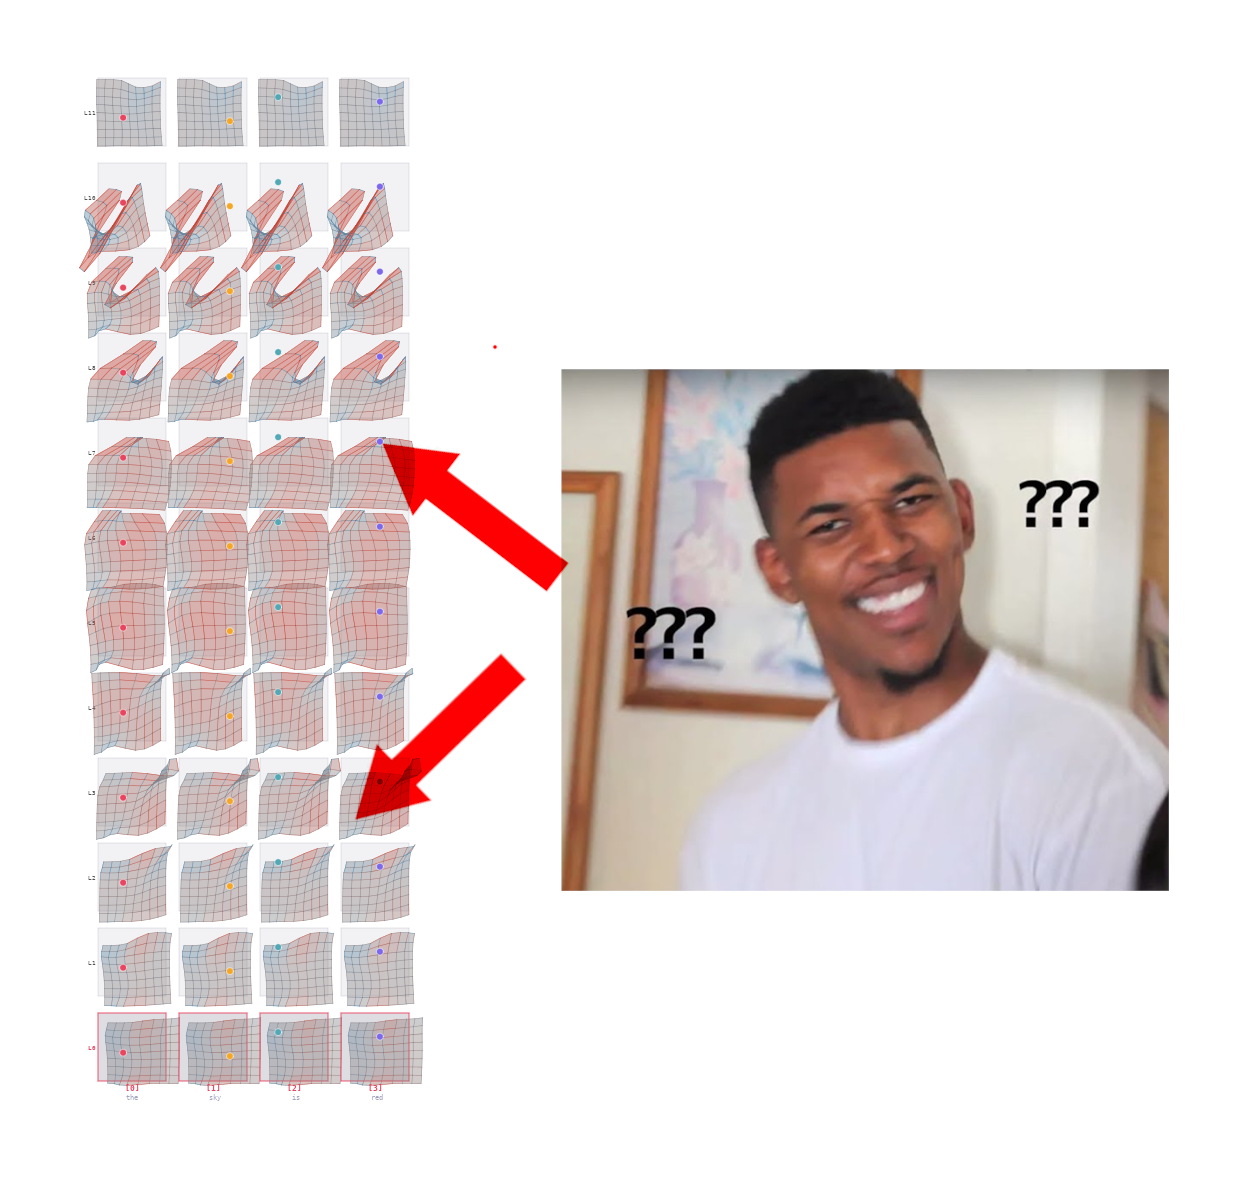
\includegraphics[width=0.75\textwidth, height=0.65\textheight, keepaspectratio]{innerlayersconfusion.png}
  \end{center}
  \vfill
\end{frame}

\begin{frame}{Können neuronale Netze \emph{rechnen}?}
  \begin{center}
    \texttt{\color{dunkel} f(x) = 2x + 5, \quad f(5) = \color{highlight}\textbf{15}}
  \end{center}

  \begin{itemize}
    \stich{Fakten speichern → klar, ist ``nur'' Kompression}
    \stich{Aber: \textbf{Algorithmen ausführen}?}
    \stich{Klappt nicht immer, nicht für alle Algorithmen …}
    \stich{… aber \emph{oft genug}, dass es kein Zufall sein kann}
    \stich{Wie bildet ein Netz aus Matrixmultiplikationen + ReLU
           eine \emph{Berechnung} ab?}
  \end{itemize}

  \medskip
  \begin{center}
    \color{akzent}\textbf{→ Meine Forschungsfrage. Hier meine spekulativen Ideen.}
  \end{center}
\end{frame}

% ============================================================
\section{Raumkrümmung}
% ============================================================

\abschnitt{Schritt 4}{Raumkrümmung – eine andere Perspektive}

\begin{frame}{Zwei Interpretationen}
  \begin{columns}[T]
    \column{0.45\textwidth}
    \begin{center}
      \textbf{Interpretation A}\\
      {\small Punkte werden \textbf{verschoben}}\\[0.3em]
      {\scriptsize (Vorher → Nachher)}
    \end{center}
    \begin{tikzpicture}[scale=0.65]
      % --- VORHER: flaches Gitter mit Punkten ---
      \draw[step=1, gray!30, thin] (-0.5,-0.5) grid (4.5,4.5);
      
      % Punkte vorher (helle Farbe)
      \fill[hell!50] (1,1) circle (5pt);
      \fill[hell!50] (3,1) circle (5pt);
      \fill[hell!50] (1,3) circle (5pt);
      \fill[hell!50] (3,3) circle (5pt);
      \fill[hell!50] (2,2) circle (5pt);
      
      % Punkte nachher (kräftige Farbe)
      \fill[akzent] (1.8,2.2) circle (5pt);
      \fill[akzent] (3.5,2.0) circle (5pt);
      \fill[akzent] (1.5,3.8) circle (5pt);
      \fill[akzent] (3.8,3.5) circle (5pt);
      \fill[akzent] (2.8,2.8) circle (5pt);
      
      % Pfeile
      \draw[-{Stealth}, thick, dashed, gray] (1,1) -- (1.8,2.2);
      \draw[-{Stealth}, thick, dashed, gray] (3,1) -- (3.5,2.0);
      \draw[-{Stealth}, thick, dashed, gray] (1,3) -- (1.5,3.8);
      \draw[-{Stealth}, thick, dashed, gray] (3,3) -- (3.8,3.5);
      \draw[-{Stealth}, thick, dashed, gray] (2,2) -- (2.8,2.8);
      
      \node[font=\scriptsize, below] at (2,-0.8) {Raum bleibt flach};
      \node[font=\scriptsize, below] at (2,-1.3) {Punkte bewegen sich};
    \end{tikzpicture}

    \column{0.45\textwidth}
    \begin{center}
      \textbf{Interpretation B}\\
      {\small Der \textbf{Raum} wird verformt}\\[0.3em]
      {\scriptsize (Vorher/Nachher = Krümmung)}
    \end{center}
    \begin{tikzpicture}[scale=0.65]
      % --- Gekrümmtes Gitter: Punkte bleiben an "gleichen Koordinaten" ---
      % --- aber Abstände haben sich verändert ---
      
      % Gekrümmtes Gitter (horizontal)
      \draw[gray!40, thin] plot[smooth] coordinates 
        {(0,0.1) (1,0.0) (2,0.2) (3,0.1) (4,0.05)};
      \draw[gray!40, thin] plot[smooth] coordinates 
        {(0.1,1.0) (1,0.85) (2,1.1) (3,0.9) (4,1.0)};
      \draw[gray!40, thin] plot[smooth] coordinates 
        {(0.0,2.0) (1,2.2) (2,2.4) (3,2.1) (4,2.0)};
      \draw[gray!40, thin] plot[smooth] coordinates 
        {(0.1,3.0) (1,3.1) (2,3.3) (3,3.0) (4,3.05)};
      \draw[gray!40, thin] plot[smooth] coordinates 
        {(0.0,4.0) (1,3.9) (2,4.1) (3,4.0) (4,3.95)};
      
      % Gekrümmtes Gitter (vertikal)
      \draw[gray!40, thin] plot[smooth] coordinates 
        {(0.0,0.1) (0.1,1.0) (0.0,2.0) (0.1,3.0) (0.0,4.0)};
      \draw[gray!40, thin] plot[smooth] coordinates 
        {(1,0.0) (1,0.85) (1,2.2) (1,3.1) (1,3.9)};
      \draw[gray!40, thin] plot[smooth] coordinates 
        {(2,0.2) (2,1.1) (2,2.4) (2,3.3) (2,4.1)};
      \draw[gray!40, thin] plot[smooth] coordinates 
        {(3,0.1) (3,0.9) (3,2.1) (3,3.0) (3,4.0)};
      \draw[gray!40, thin] plot[smooth] coordinates 
        {(4,0.05) (4,1.0) (4,2.0) (4,3.05) (4,3.95)};
      
      % Punkte an "gleichen" Gitterkoordinaten – aber Raum ist verzerrt
      \fill[hell] (1,0.85) circle (5pt);
      \fill[hell] (3,0.9) circle (5pt);
      \fill[hell] (1,3.1) circle (5pt);
      \fill[hell] (3,3.0) circle (5pt);
      \fill[hell] (2,2.4) circle (5pt);
      
      % Abstandsannotation: zeige dass Abstände sich geändert haben
      \draw[akzent, thick, {Stealth}-{Stealth}] (1,0.85) -- (2,2.4)
        node[midway, left, font=\tiny\color{akzent}] {nah};
      \draw[highlight, thick, {Stealth}-{Stealth}] (3,0.9) -- (2,2.4)
        node[midway, right, font=\tiny\color{highlight}] {weit};
      
      \node[font=\scriptsize, below] at (2,-0.8) {Punkte bleiben};
      \node[font=\scriptsize, below] at (2,-1.3) {Raum speichert die Info};
    \end{tikzpicture}
  \end{columns}

  \medskip
  \begin{itemize}
    \stich{Links: gleiche Transformation für alle → \textbf{keine} Strukturinfo}
    \stich{Rechts: Krümmung verändert \textbf{Abstände nicht-uniform} → Information steckt im Raum}
    \stich{Krümmung = \textbf{differentielle} Information: ``hier dichter, dort weiter''}
  \end{itemize}
\end{frame}

% ============================================================
\section{Topologie}
% ============================================================

\abschnitt{Schritt 5}{Topologie – Geometrie ohne Distanz}

\begin{frame}{Was ist Topologie?}
  \begin{columns}[T]
    \column{0.55\textwidth}
    \begin{itemize}
      \stich{Geometrie von Oberflächen – aber \textbf{ohne konkrete Distanzen}}
      \stich{Nur noch: $d(x,y)$ – abstrakte Metrik\\
             {\small (im normalen Raum: Pythagoras)}}
      \stich{KI: es geht um \textbf{Relationen}, nicht um absolute Abstände}
      \stich{Daher: \textbf{topologische Form} des Embedding-Raums ist entscheidend}
    \end{itemize}

    \column{0.4\textwidth}
    \placeholder[0.9\linewidth]{Meme: Topologe kann Kaffeetasse
                                 nicht von Donut unterscheiden}
  \end{columns}

  \medskip
  \begin{center}
    \begin{tikzpicture}[scale=0.6]
      % Torus
      \draw[thick, dunkel] (0,0) ellipse (2 and 0.8);
      \draw[thick, dunkel] (-0.7,0.1) arc (180:360:0.7 and 0.3);
      \draw[thick, dunkel, dashed] (-0.7,0.1) arc (180:0:0.7 and 0.3);
      \node[below, font=\small] at (0,-1.2) {Torus (Donut)};

      % Hose
      \begin{scope}[xshift=6cm]
        \draw[thick, dunkel] (-1,1.5) to[out=-90,in=180] (0,0)
          to[out=0,in=-90] (1,1.5);
        \draw[thick, dunkel] (-1,1.5) arc (180:360:1 and 0.3);
        \draw[thick, dunkel] (0,0) to[out=-150,in=90] (-0.8,-1.5);
        \draw[thick, dunkel] (0,0) to[out=-30,in=90] (0.8,-1.5);
        \draw[thick, dunkel] (-0.8,-1.5) arc (180:360:0.4 and 0.15);
        \draw[thick, dunkel] (0.4,-1.5) arc (180:360:0.4 and 0.15);
        \node[below, font=\small] at (0,-2) {Topologische Hose};
      \end{scope}
    \end{tikzpicture}
  \end{center}
\end{frame}

% ── Loop Spaces ────────────────────────────────────────────
\begin{frame}{Loop Spaces – Topologie kann rechnen}
  \begin{columns}[T]
    \column{0.55\textwidth}
    \begin{itemize}
      \stich{\textbf{Loop Space:} Raum aller geschlossenen Pfade auf einer Fläche}
      \stich{Ein Pfad = eine Zahl\\
             Anderer Pfad = andere Zahl}
      \stich{Verkettung von Pfaden $\sim$ Addition}
      \stich{Umkehrrichtung $\sim$ Subtraktion (Minus)}
      \stich{Pfad und Rechnung sind \textbf{homotop} – ineinander überführbar}
    \end{itemize}

    \medskip
    {\small\color{gray} Anwendung: automatisches Beweisen
     (Homotopie-Typentheorie)}

    \column{0.4\textwidth}
    \placeholder[0.9\linewidth]{GIF / Bild: Loop Space beim Zählen –
                                 Schleifen werden verkettet}
  \end{columns}
\end{frame}

% ============================================================
\section{Holografische Kodierung}
% ============================================================

\abschnitt{Schritt 6}{Holografische Kodierung}

\begin{frame}{Pigeonhole-Prinzip \& verteilte Speicherung}
  \begin{columns}[T]
    \column{0.5\textwidth}
    \begin{itemize}
      \stich{\textbf{Mehr Konzepte als Neuronen}\\
             → ein Neuron speichert \emph{mehrere} Konzepte}
      \stich{Kein ``Großmutter-Neuron''\\
             {\small (kein einzelnes Neuron = ein Konzept)}}
      \stich{Information \textbf{verteilt} über das gesamte Netz}
      \stich{Wie ein \textbf{Hologramm}: jedes Fragment enthält
             das ganze Bild (unscharf)}
    \end{itemize}

    \column{0.45\textwidth}
    \begin{center}
      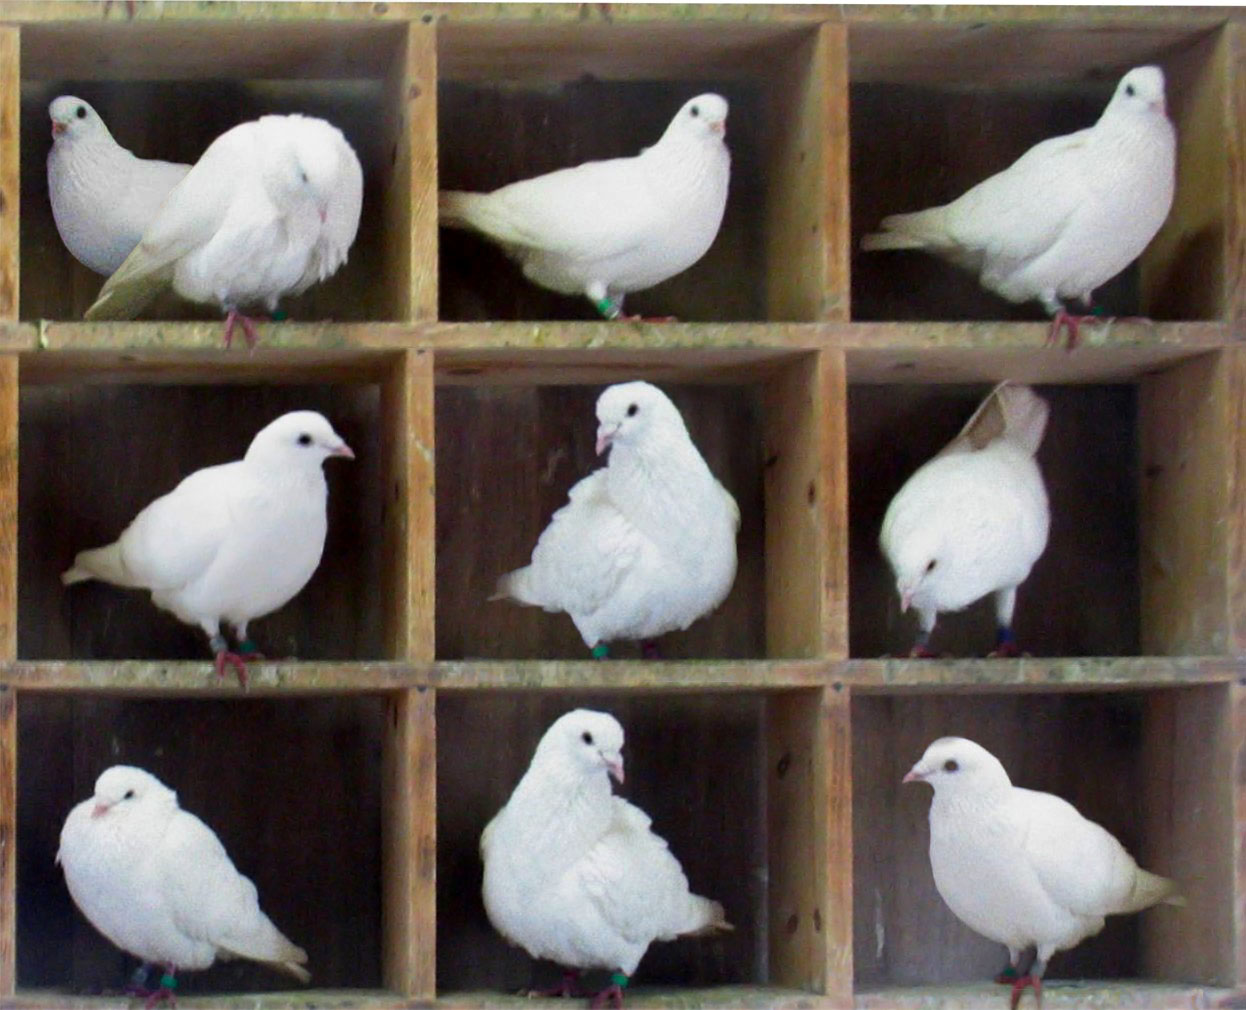
\includegraphics[width=0.9\linewidth]{pidgeonhole_principle.jpg}\\
      {\scriptsize\color{gray}Pigeonhole-Prinzip: mehr Tauben als Löcher}
    \end{center}
  \end{columns}
\end{frame}

\begin{frame}{Holografische Kodierung}
  \begin{columns}[T]
    \column{0.48\textwidth}
    \begin{center}
      
\includegraphics[width=0.9\linewidth, height=0.4\textheight, keepaspectratio]{hologram1.png}\\
      {\scriptsize\color{gray}Originalbild (z.\,B.\ Smiley)}
    \end{center}

    \column{0.48\textwidth}
    \begin{center}
      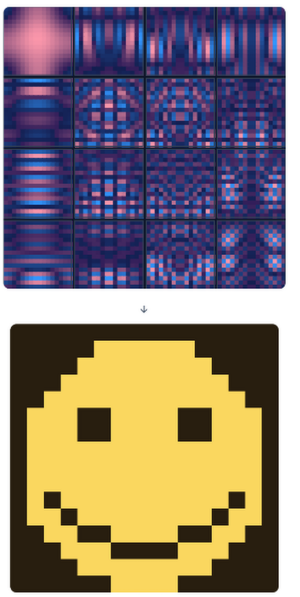
\includegraphics[width=0.9\linewidth, height=0.4\textheight, keepaspectratio]{hologram2.png}\\
      {\scriptsize\color{gray}Holografisches Interferenzmuster}
    \end{center}
  \end{columns}

  \medskip
  \begin{itemize}
    \stich{Links: das gespeicherte \textbf{Konzept} (lokalisiert, klar)}
    \stich{Rechts: die \textbf{verteilte Kodierung} im Netz (jedes Fragment enthält Information über das Ganze)}
    \stich{Zerstört man einen Teil des Hologramms → Bild wird \emph{unschärfer}, aber nicht gelöscht}
    \stich{Analog: einzelne Neuronen entfernen → Modell degradiert \emph{graduell}}
  \end{itemize}
\end{frame}

\begin{frame}{Holografische Kodierung}
  \begin{columns}[T]
    \column{0.48\textwidth}
    \begin{center}
      
\includegraphics[width=0.85\linewidth, height=0.35\textheight, keepaspectratio]{hologram1_1.png}\\[0.3em]
      {\scriptsize\color{gray}Ein Stück herausgeschnitten\\→ Information \textbf{unwiederbringlich weg}}
    \end{center}

    \column{0.48\textwidth}
    \begin{center}
      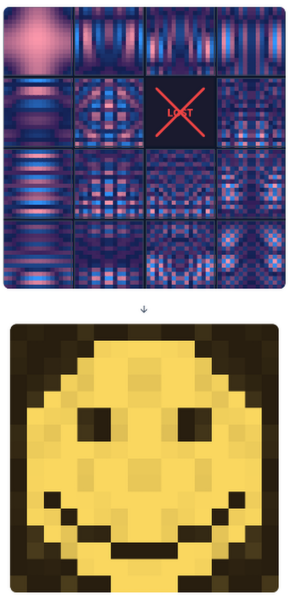
\includegraphics[width=0.85\linewidth, height=0.35\textheight, keepaspectratio]{hologram2_2.png}\\[0.3em]
      {\scriptsize\color{gray}Ein Stück herausgeschnitten\\→ Bild wird \textbf{unschärfer}, aber bleibt ganz}
    \end{center}
  \end{columns}

  \medskip
  \begin{itemize}
    \stich{\textbf{Links:} Lokale Speicherung – jeder Pixel trägt nur \emph{seine eigene} Information. Teil weg = Loch im Bild.}
    \stich{\textbf{Rechts:} Verteilte Speicherung – jedes Fragment enthält Information über das \emph{gesamte} Bild. Teil weg = alles etwas unschärfer.}
    \stich{Neuronale Netze speichern wie \textbf{Hologramme}: einzelne Neuronen entfernen → gradueller Qualitätsverlust, kein katastrophales Vergessen}
  \end{itemize}

  \quelle{Vgl.\ Holografie: jeder Teil des Hologramms rekonstruiert das ganze Bild}
\end{frame}

\begin{frame}{Raumkrümmung + Holografie = Berechnung?}
  \begin{center}
    \begin{tikzpicture}[
        box/.style={draw, thick, rounded corners, minimum width=3.5cm,
                     minimum height=1cm, font=\small\bfseries, text=white},
        arr/.style={-{Stealth}, thick, akzent}
      ]
      \node[box, fill=dunkel]    (krumm) at (0,2)   {Raumkrümmung};
      \node[box, fill=hell]      (holo)  at (0,0)   {Holografische Kodierung};
      \node[box, fill=highlight] (loop)  at (0,-2)  {Loop Spaces / Topologie};

      \draw[arr] (krumm) -- node[right, font=\scriptsize, text=black]
        {enthält Info} (holo);
      \draw[arr] (holo) -- node[right, font=\scriptsize, text=black]
        {ermöglicht Rechnung} (loop);

      \draw[arr, dashed] (loop.west) to[out=180, in=180] node[left, font=\scriptsize, text=black]
        {Jacobi-Felder?} (krumm.west);
    \end{tikzpicture}
  \end{center}

  \begin{itemize}
    \stich{\textbf{Hypothese:} Die holografisch kodierte Berechnung findet
           \emph{in} der Raumkrümmung statt}
    \stich{Physikalische Methoden (Jacobi-Felder) → Zugang zur internen Geometrie}
    \stich{Ziel: Loop Spaces oder andere topologische Strukturen dort nachweisen}
  \end{itemize}
\end{frame}

% ============================================================
\section{Garbentheorie}
% ============================================================

\abschnitt{Schritt 7}{Garbentheorie – lokale Daten, globales Bild}

\begin{frame}[plain]
  \begin{center}
    {\Huge\color{dunkel}\textbf{Garbentheorie}}\\[1em]
    {\large Wie fügt man lokale Beobachtungen zu einem kohärenten Ganzen?}
  \end{center}

  \vspace{1em}
  \placeholder[0.6\textwidth]{Bildseite: Garbentheorie-Illustration}
\end{frame}

\begin{frame}{Situs – ein Ort für Messungen}
  \begin{itemize}
    \stich{\textbf{Situs} = etwas, an dem man Untersuchungen anstellen kann}
    \stich{Beispiele: Temperatur messen, Farbe bestimmen, Größe schätzen …}
    \stich{Lokale Messungen → versuchen, zu einem \textbf{kohärenten Bild} zusammenzufügen}
  \end{itemize}

  \medskip
  \begin{center}
    \begin{tikzpicture}[scale=0.8]
      % Überlappende Kreise
      \fill[hell!20] (0,0) circle (1.8);
      \fill[akzent!20] (2.2,0) circle (1.8);
      \fill[highlight!30] (1.1,0) ellipse (0.7 and 1.2);

      \node[font=\small] at (-0.5,0) {Messung A};
      \node[font=\small] at (2.7,0) {Messung B};
      \node[font=\scriptsize\color{highlight}] at (1.1,-0.3) {Überlappung};

      % Annotation
      \draw[{Stealth}-, thick, gray] (1.1, 1.4) -- ++(0, 0.8)
        node[above, font=\scriptsize, text width=3cm, align=center]
        {Hier müssen sie\\übereinstimmen!};
    \end{tikzpicture}
  \end{center}
\end{frame}

\begin{frame}{Panorama-Prinzip}
  \begin{columns}[T]
    \column{0.55\textwidth}
    \begin{itemize}
      \stich{Verschiedene \textbf{Perspektiven} auf die Welt}
      \stich{Realer Sachverhalt → Perspektiven \textbf{müssen überlappen}}
      \stich{Überlappung = Verklebungsbedingung}
      \stich{Wenn sie \emph{nicht} überlappen → \textbf{nicht verklebbar}}
    \end{itemize}

    \medskip
    {\small Wie beim Handy-Panorama: Bilder werden an den
     Überlappungen zusammengefügt.}

    \column{0.4\textwidth}
    \placeholder[0.9\linewidth]{Bild: Handy-Panorama mit sichtbarer
                                 Überlappung der Einzelbilder}
  \end{columns}
\end{frame}

\begin{frame}{Der Situs der KI}
  \begin{itemize}
    \stich{Situs der KI = Texte von Menschen über \textbf{die Welt}}
    \stich{Aber: sie sieht die Welt nur durch \textbf{kleine Schnitte}
           (= Worte aus Texte aus dem Training im Kontext)}
    \stich{Im Internet steht ``alles und das Gegenteil von allem''\\
           → \textbf{nicht global verklebbar}}
    \stich{Aber \textbf{lokal} durchaus verklebbar → \emph{lokale Garben}}
  \end{itemize}

  \medskip
  \begin{center}
    \begin{tikzpicture}[scale=0.7]
      % "Welt" als großer Kreis
      \draw[thick, dunkel, dashed] (0,0) circle (3);
      \node[font=\small\color{dunkel}] at (0,-3.5) {Die Welt (Situs)};

      % Kleine "Halme" (Texte)
      \foreach \angle/\col in {30/hell, 80/akzent, 140/highlight,
                                200/hell, 260/akzent, 320/highlight} {
        \fill[\col!30] (\angle:2.2) circle (0.6);
        \draw[\col, thick] (\angle:2.2) circle (0.6);
      }

      % Einige überlappen
      \node[font=\tiny] at (55:2.2) {$\cap$};
      \node[font=\tiny] at (110:2.2) {$\cap$};

      % Annotation
      \node[font=\scriptsize, text width=2.5cm, align=center] at (5,1)
        {Texte = lokale\\Schnitte auf\\dem Situs};
    \end{tikzpicture}
  \end{center}
\end{frame}

\begin{frame}{Keime, Muster, Generierung}
  \begin{itemize}
    \stich{KI lernt auf diesen \textbf{Keimen} (lokalen Daten) Muster zu erkennen}
    \stich{Ziel: neue Keime \textbf{dynamisch generieren} können}
    \stich{Wie? Indem sie in den Raumkrümmungen \textbf{topologische Strukturen}
           aufbaut}
    \stich{Diese sind \textbf{approximative Muster} der realen Welt}
  \end{itemize}

  \medskip
  \begin{center}
    \begin{tikzpicture}[
        arr/.style={-{Stealth}, thick, akzent}
      ]
      \node[draw, rounded corners, fill=hell!15, minimum width=2cm,
            font=\small\bfseries] (attn) at (0,0) {Attention Heads};
      \node[draw, rounded corners, fill=akzent!15, minimum width=2cm,
            font=\small\bfseries] (ffn) at (5,0) {FFN};
      \node[font=\scriptsize, text width=3cm, align=center, below=0.3cm of attn]
        {Lesen: wo ist die\\aktuelle Bedeutung?};
      \node[font=\scriptsize, text width=3cm, align=center, below=0.3cm of ffn]
        {Erstellen: neue\\topologische Strukturen};
      \draw[arr] (attn) -- node[above, font=\scriptsize] {Info} (ffn);
    \end{tikzpicture}
  \end{center}
\end{frame}

% ── Tegmark: Space & Time ──────────────────────────────────
\begin{frame}{Evidenz: Modelle lernen Geografie}
  \begin{columns}[T]
    \column{0.55\textwidth}
    \begin{itemize}
      \stich{Gurnee \& Tegmark (2023):\\
             \emph{``Language Models Represent Space and Time''}}
      \stich{Abstände zwischen Städten (New York, Berlin, …)
             in einer Dimension \textbf{realistisch} abgebildet}
      \stich{Nicht explizit trainiert – emergiert als
             \textbf{beste Repräsentation} der Daten}
    \end{itemize}

    \column{0.4\textwidth}
    \placeholder[0.9\linewidth]{Bild: Tegmark – interne Geografie-Karte
                                 des Sprachmodells}
  \end{columns}

  \quelle{Gurnee, Tegmark. arXiv:2310.02207 (2023)}
\end{frame}

\begin{frame}{Warum lernt das Modell Geografie?}
  \formelbox{\text{Strukturelle Kompression} \gg \text{Einzelverbindungen}}

  \begin{itemize}
    \stich{\textbf{Strukturelle Kompression:}\\
           Ein kohärentes 2D/3D-Koordinatensystem ist ``billiger''
           als Milliarden Einzelverbindungen zwischen Städten}
    \stich{\textbf{Generalisierung:}\\
           ``A östlich von B'' + ``B östlich von C''
           → automatisch auf einer Linie angeordnet}
    \stich{Erlaubt Antworten auf Fragen, die \textbf{nie im Training} vorkamen}
  \end{itemize}
\end{frame}

\begin{frame}{Prä-Garbe, nicht Garbe}
  \begin{center}
    \begin{tikzpicture}
      \node[draw, thick, rounded corners, fill=highlight!10,
            minimum width=8cm, minimum height=2cm, font=\large\bfseries]
        {Die Daten bleiben \textbf{Approximationen}.};
    \end{tikzpicture}
  \end{center}

  \begin{itemize}
    \stich{Nicht ``verstanden'' (dann wäre es eine \textbf{Garbe})}
    \stich{Bleibt eine \textbf{Prä-Garbe} aus lokalen Daten}
    \stich{Auch lokal nicht immer verklebbar (Widersprüche im Training)}
    \stich{Von konkreter Hardware abhängig, \tt{float}-Berechnungen haben nur begrenzte Genauigkeiten.}
    \stich{Daher: KI kann sich irren, halluzinieren, inkonsistent sein}
  \end{itemize}
\end{frame}

% ============================================================
\section{Zusammenfassung}
% ============================================================

\abschnitt{Zusammenfassung}{Das Gesamtbild}

\begin{frame}{Der Fluss – von Tokens zu Topologie}
  \begin{center}
    \begin{tikzpicture}[
        box/.style={draw, thick, rounded corners, minimum width=2.6cm,
                     minimum height=0.65cm, font=\tiny\bfseries},
        layer/.style={draw, thick, rounded corners, minimum width=2.6cm,
                     minimum height=0.65cm, font=\tiny\bfseries,
                     fill=dunkel!15, text=black},
        arr/.style={-{Stealth}, thick, gray},
        note/.style={font=\tiny, text width=2.6cm, align=center},
        node distance=0.3cm and 0.4cm
      ]
      % ── Zeile 1: Eingang ──
      \node[box, fill=hell!15]                             (tok) {Tokenizer};
      \node[box, fill=hell!15, right=of tok]               (emb) {Embedding};
      \node[box, fill=hell!25, right=of emb]               (pos) {+ Pos.\ Encoding};
      \node[layer, right=of pos]                           (res) {Residual Stream};

      \foreach \a/\b in {tok/emb, emb/pos, pos/res}
        \draw[arr] (\a) -- (\b);

      % ── Zeile 2: Transformer-Block (×N) ──
      \node[layer, below=1.0cm of tok]                     (attn){Attention};
      \node[layer, right=of attn]                          (ffn) {FFN};
      \node[box, fill=akzent!20, right=of ffn]             (curv){Raumkrümmung};
      \node[box, fill=highlight!20, right=of curv]         (out) {Topologie / Garbe};

      \foreach \a/\b in {attn/ffn, ffn/curv, curv/out}
        \draw[arr] (\a) -- (\b);

      % ── Verbindung Zeile 1 → Zeile 2 ──
      \draw[arr, rounded corners=5pt]
        (res.south) -- ++(0,-0.4) -| (attn.north);

      % ── Rückschreiben auf Residual Stream (Loop) ──
      \draw[arr, rounded corners=5pt, dashed]
        (ffn.south) -- ++(0,-0.4) -- ++(-4.2,0)
        node[midway, below, font=\tiny]{$+$ zurück auf Residual Stream ($\times N$ Layer)}
        -- ++(0,0.4) -- (attn.south west);

      % ── Annotationen ──
      \node[note, above=0.2cm of tok]  {Text → IDs};
      \node[note, above=0.2cm of pos]  {Sequenz-\\information};
      \node[note, above=0.2cm of res]  {Informations-\\autobahn};
      \node[note, below=0.2cm of curv] {Jeder Layer\\krümmt den Raum};
      \node[note, below=0.2cm of out]  {Holograf.\ kodiert,\\immer schärfere\\Garben-Approx.};
    \end{tikzpicture}
  \end{center}
\end{frame}

\begin{frame}{Offene Fragen}
  \begin{itemize}
    \stich{Können wir mit \textbf{Jacobi-Feldern} die interne Geometrie vermessen?}
    \stich{Gibt es nachweisbare \textbf{Loop Spaces} in trainierten Netzen?}
    \stich{Ist die holografische Kodierung der Schlüssel zum
           \textbf{mechanistischen Verständnis}?}
  \end{itemize}

  \vfill
  \begin{center}
    {\Large\color{akzent}\textbf{Danke!}}\\[0.5em]
    {\small Fragen?}
  \end{center}
\end{frame}

% ============================================================
\end{document}
% ============================================================
